\documentclass{article}
\usepackage[utf8]{inputenc}
\usepackage[spanish]{babel}
\usepackage{graphicx}
\usepackage{dirtytalk}
\usepackage{caratula}
\usepackage{enumerate}
\usepackage{amssymb}
\usepackage{amsmath}
\usepackage{geometry}
\usepackage{fixltx2e}
\usepackage{wrapfig}
\usepackage{verbatim}
\usepackage{cite}
\usepackage{float}
\usepackage[space]{grffile}
\geometry{
 a4paper,
 total={210mm,297mm},
 left=30mm,
 right=30mm,
 top=30mm,
 bottom=30mm,
 }
 
\begin{document}
% Estos comandos deben ir antes del \maketitle
\materia{Sistemas Operativos} % obligatorio

\titulo{Trabajo Práctico 1}
\subtitulo{}
\grupo{}

\integrante{Bayardo Julián}{850/13}{julian@bayardo.com.ar} % obligatorio
\integrante{Cuneo Christian}{755/13}{chriscuneo93@gmail.com} % obligatorio 
 
\maketitle

\pagebreak

\tableofcontents

\pagebreak

\section{Ejercicio 1}

La implementación en este caso es realmente simple: consiste simplemente en generar números aleatoriamente distribuidos utilizando el generador pseudoaleatorio de la librería estándar de C++, seedeado utilizando el tiempo UNIX en el que se corre el algoritmo. Elegimos utilizar C++11 para esto precisamente porque utilizar la clásica función random de la librería en las versiones anteriores es problemático para generar números entre cierto rango, como es pedido en el enunciado. Podemos observar en la figura \ref{grf:ex1} el resultado de evaluar un lote de \verb`TaskConsola 10 2 20`

\begin{figure}[h!]
\caption{Lote de tareas que utiliza TaskConsola \label{grf:ex1}}
\centering
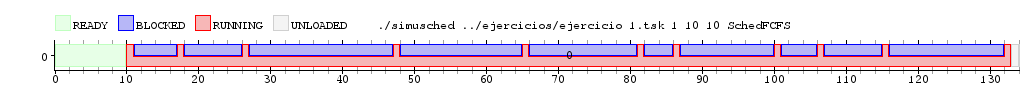
\includegraphics[width=15cm]{../ejercicios/ejercicio 1}
\end{figure}

\section{Ejercicio 2}



\begin{figure}[h!]
\caption{Lote de tareas ejecutándose en 1 núcleo \label{grf:ex2-1}}
\centering
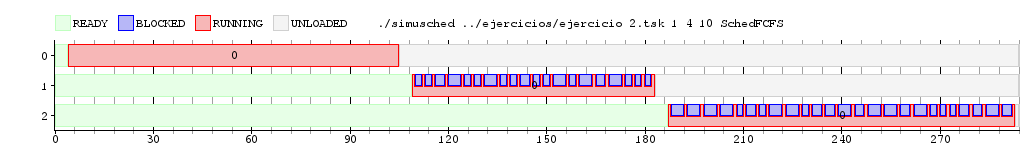
\includegraphics[width=15cm]{../ejercicios/ejercicio 2 - 1 nucleo}
\end{figure}

\begin{figure}[h!]
\caption{Lote de tareas ejecutándose en 2 núcleos \label{grf:ex2-2}}
\centering
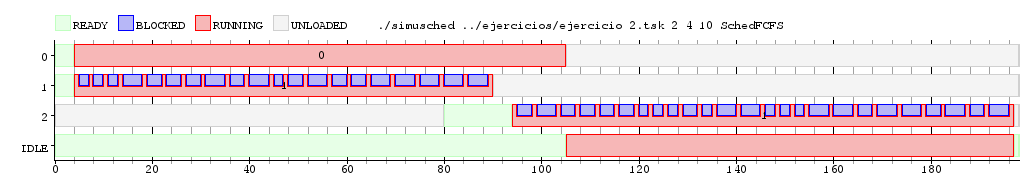
\includegraphics[width=15cm]{../ejercicios/ejercicio 2 - 2 nucleos}
\end{figure}

\section{Ejercicio 3}
\section{Ejercicio 4}
\section{Ejercicio 5}
\section{Ejercicio 6}
\section{Ejercicio 7}
\section{Ejercicio 8}

\end{document}